\documentclass[11pt,spanish]{article}
\usepackage[spanish]{babel}
\selectlanguage{spanish}
\usepackage[utf8]{inputenc}
\DeclareUnicodeCharacter{2212}{-}
\DeclareUnicodeCharacter{2265}{+}
\usepackage{graphicx}
\usepackage{mathtools}
\usepackage{amssymb}
\usepackage{xcolor}
\usepackage{float}
\usepackage{hyperref}
\usepackage{subfigure}
\usepackage{geometry}
 \geometry{
 a4paper,
 total={170mm,257mm},
 left=20mm,
 top=20mm,
 }

%Use \href{URL}{DESCRIPTION} to add a link with description.
%Use \url{URL} to add a link without a description.



\title{Spotify}
\date{2021-10-01}
\author{Abraham Corta Ramírez y José Calcedo Vázquez}

\begin{document}
\pagenumbering{gobble}
\maketitle
\newpage
\pagenumbering{arabic}

\tableofcontents

\listoffigures

\clearpage

\section{Introducción a Spotify}

\paragraph*{Para este trabajo de programación la plataforma que vamos a utilizar es Spotify, esta aplicación es empleada para la reproducción de música vía streaming. Actualmente Spotify es uno de los líderes del sector y contiene millones de canciones y cientos de miles de artistas de todos los géneros.}

\paragraph*{Spotify ofrece una \href{https://developer.spotify.com/documentation/web-api/}{Web API} con la que nos permite acceder a numerosos datos como canciones, artistas, playlists, etc. Y no solo eso, sino que de una canción en concreto se pueden obtener datos como su tempo, la duración, su grado de «instrumentalidad», de energía, etc. Esta API se puede utilizar con diferentes lenguajes como PHP, Java, JavaScript o Python entre otras mediante el uso de librerías.}

\paragraph*{Nosotros hemos decido hacerlo con Python debido a que es mas ligero que Java y más simple de utilizar.}

\paragraph*{La API se compone de muchos componentes, a continuación, se nombran algunos de estos:}

\begin{itemize}
	\item \textbf{Peticiones}
	\item \textbf{Spotify URls e IDs }
	\item \textbf{Respuestas: en formato JSON}
	\item \textbf{Paginación}
	\item \textbf{Autenticación }
\end{itemize}

\paragraph*{Nuestro objetivo será manipular los datos de la API sobre un artista en concreto, y partiendo de ahí estudiaremos sus conexiones, los artistas relacionados y las playlists.}

\paragraph*{El primer paso es crearnos \href{https://developer.spotify.com/dashboard/applications}{una cuenta como desarrollador Spotify}, 
	si ya tenemos cuenta de Spotify solo necesitaremos iniciar sesión en la web de desarrolladores. Será necesario dar de alta una aplicación, de esta manera obtendremos un Client ID y un Client Secret.
	Veasé las siguientes figuras: \footnote{Se han ocultado los client ID de las figuras ya que este puede ser usado por cualquier persona.}}

\begin{figure}[h!]
    \centering
    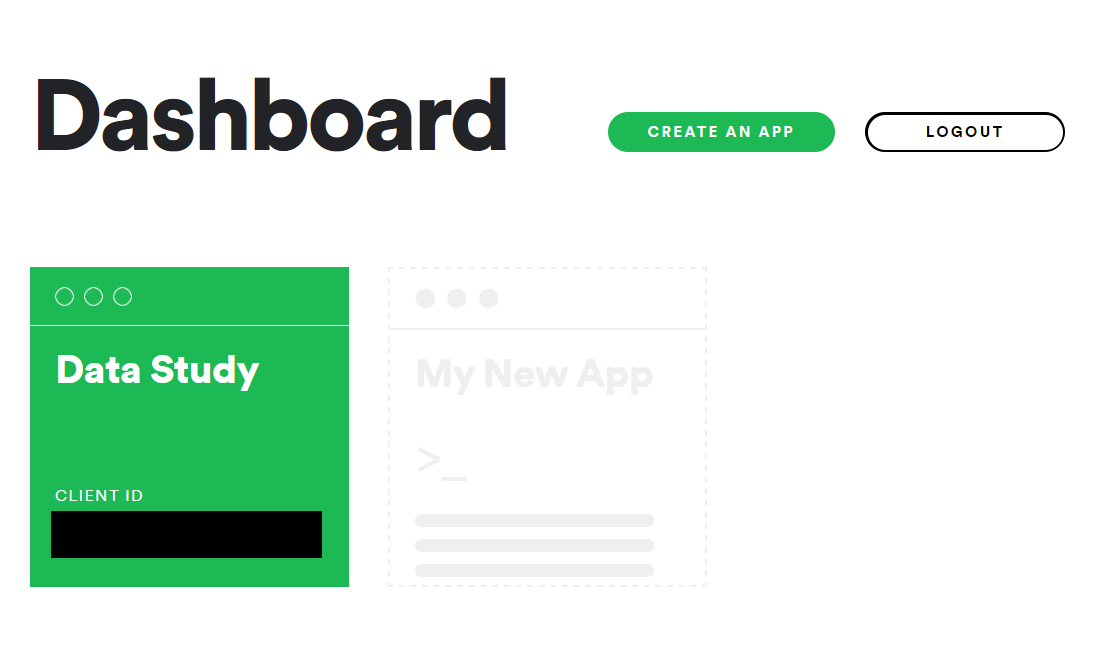
\includegraphics[width=120mm]{spotify_dev_dashboard.png}
    \caption{Spotify dashboard}
\end{figure}

\begin{figure}[h!]
    \centering
	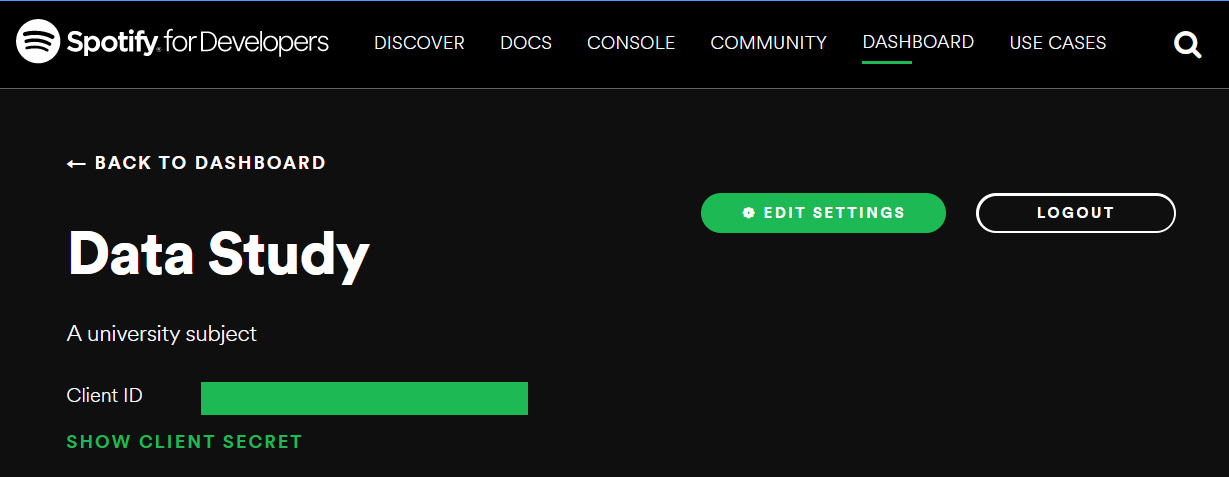
\includegraphics[width=120mm]{devoloper_spotify_1.png}
    \caption{Spotify application}
\end{figure}

\paragraph*{Una vez tengamos nuestra aplicacion creada necesitaremos el client ID y el client secret para poder autenticarnos 
y recuperar datos de la API.}

\paragraph*{Nuestro trabajo se compone de dos programas, el primero escrito en python utilizando Visual Studio Code
que nos permite recuperar datos de la API de Spotify y exportarlos a JSON. 
Y el segundo escrito en SageMath que nos permite representar y estudiar esos datos con teoría de grafos.}

\section{Código Python}

\paragraph*{El codigo python se compone de tres secciones}
\begin{itemize}
	\item \textbf{Conexion}
	\item \textbf{Recolección de datos}
	\item \textbf{Exportación}
\end{itemize}

\paragraph*{Para que el codigo funcione solo se han necesitado 3 librerias:}
\begin{itemize}
	\item \textbf{spotipy.oauth2-SpotifyClientCredentials:} nos permite hacer la autenticación.
	\item \textbf{pandas:} que nos permite crear los dataframes que vamos a exportar a SageMath.
	\item \textbf{spotipy:} nos permite interactuar con la API.
\end{itemize}
\paragraph*{A continuación se explicaran las imagenes presentes en la figura~\ref{fig:codigoPython}.}


\paragraph*{Lo primero que hacemos es obtener todas las playlists relacionadas con el artista. Para ello hemos tomado la URL de cada una de las playlists de 50 Cent y las hemos almacenado para su posterior uso. 
Tras ello, para cada playlist llamamos al comando sp.user\textunderscore playlist, que nos permite obtener los datos de una playlist dada su URL, para más tarde almacenar las canciones que contiene cada una.}

\paragraph*{Una vez obtenidas las canciones, creamos un bucle con el que para cada canción que hayamos obtenido, obtenemos primeramente un dataset de las playlists, donde metemos los nombres de las canciones junto al nombre de sus artistas. 
Tras hacer eso, creamos un dataset con los artistas, obteniendo su nombre, géneros musicales asociados, popularidad y seguidores con el comando sp.artist. }

\paragraph*{Finalmente, convertimos los datasets obtenidos anteriormente en Data Frames usando pandas (en el código lo usamos como pd) que posteriormente son procesados en formato JSON con el comando .to\textunderscore json, al cual le pasamos como argumento la ubicación de donde va a terminar el fichero con los datos y el dataframe correspondiente. }

\pagebreak
\begin{figure}[H]
	\begin{center}
%
	   \subfigure[conexion API]{%
		   \label{fig:first}
		   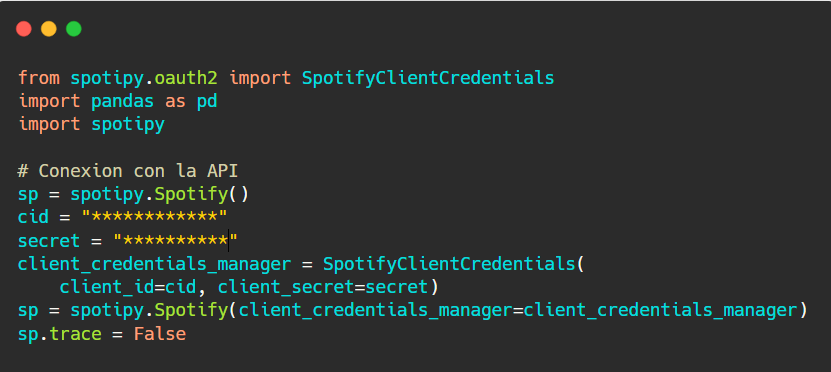
\includegraphics[width=0.7\textwidth]{programa_1.png}
	   }%
	   
	   \subfigure[Urls que utilizaremos con la API]{%
		   \label{fig:second}
		   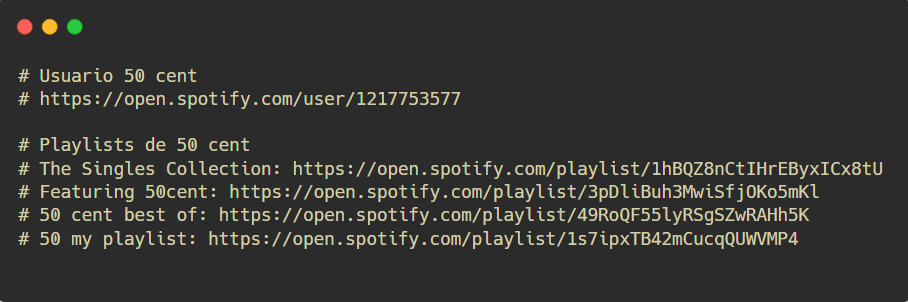
\includegraphics[width=0.7\textwidth]{programa_2.png}
	   }\\ %  ------- End of the first row ----------------------%
	   \subfigure[Recolección y exportación de los datos]{%
		   \label{fig:third}
		   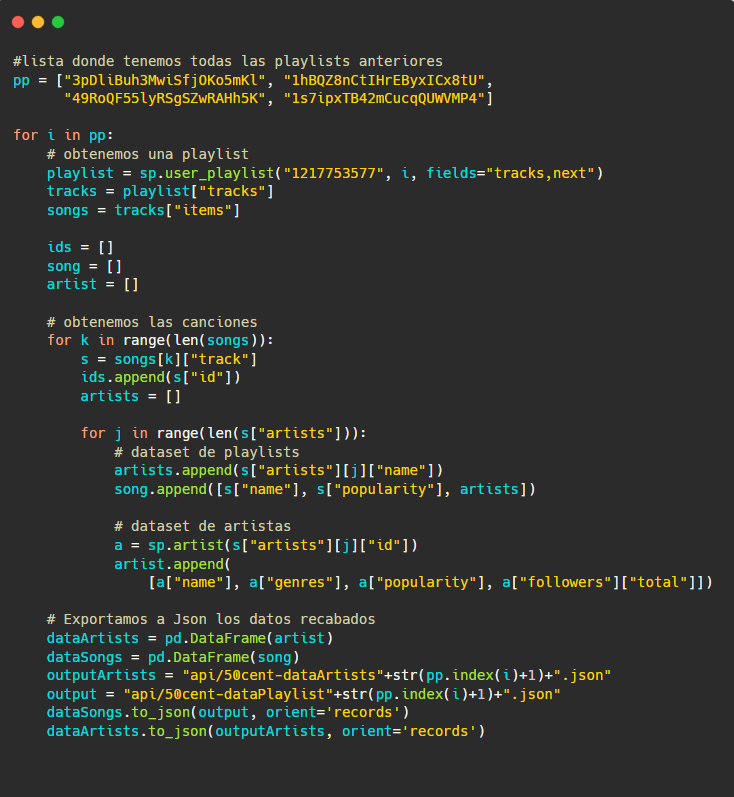
\includegraphics[width=0.7\textwidth]{programa_3.png}
	   }%
	  
%
	\end{center}
	\caption{%
	Código Python
 	}%
	\label{fig:codigoPython}
\end{figure}

\pagebreak

\section{Código SageMath}

\paragraph*{Una vez hemos extraído los datos de la API es turno de importar los datos Json, para ello utilizaremos la librería \emph{json}.}

\paragraph*{Una vez importado utilizaremos dos listas que englobaran los 4 datasets, uno para las playlist y otro para los artistas.}

\paragraph*{Para crear el grafo hemos recorrido cada Playlist y enlazado aquellos artistas que aparecen en dicha playlist, 
el resultado es un grafo en donde cada color representa una playlist y cada vértice un artista.}



\begin{figure}[H]
	\begin{center}
%
	   \subfigure[librerias json]{%
		   \label{fig:first}
		   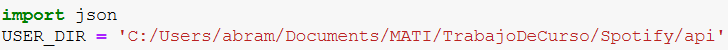
\includegraphics[width=0.7\textwidth]{sage_1.png}
	   }%
	   
	   \subfigure[importación de los datos de los artistas]{%
		   \label{fig:second}
		   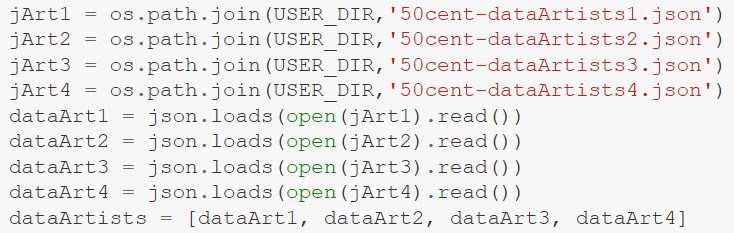
\includegraphics[width=0.7\textwidth]{sage_2.png}
	   }\\ %  ------- End of the first row ----------------------%
	   \subfigure[importación de los datos de las playlists]{%
		   \label{fig:third}
		   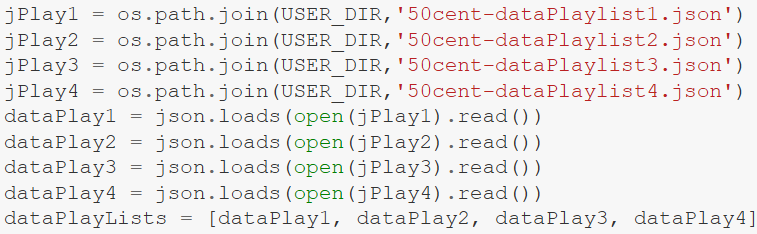
\includegraphics[width=0.7\textwidth]{sage_3.png}
	   }%
	  
%
	\end{center}
	\caption{%
	Código SageMath 1
 	}%
	\label{fig:codigoSage1}
\end{figure}

\begin{figure}[H]
	\begin{center}
%
	   \subfigure[metódos auxiliares para crear el grafo]{%
		   \label{fig:first}
		   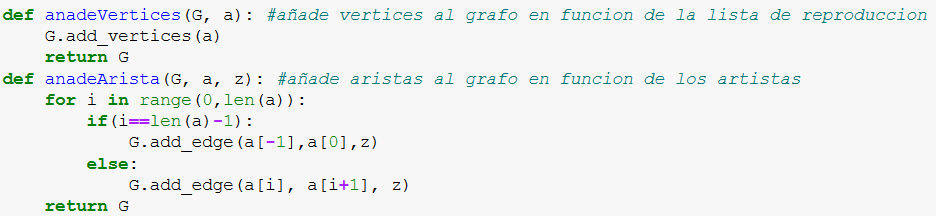
\includegraphics[width=0.7\textwidth]{sage_5.png}
	   }%
	   
	   \subfigure[creación del grafo]{%
		   \label{fig:second}
		   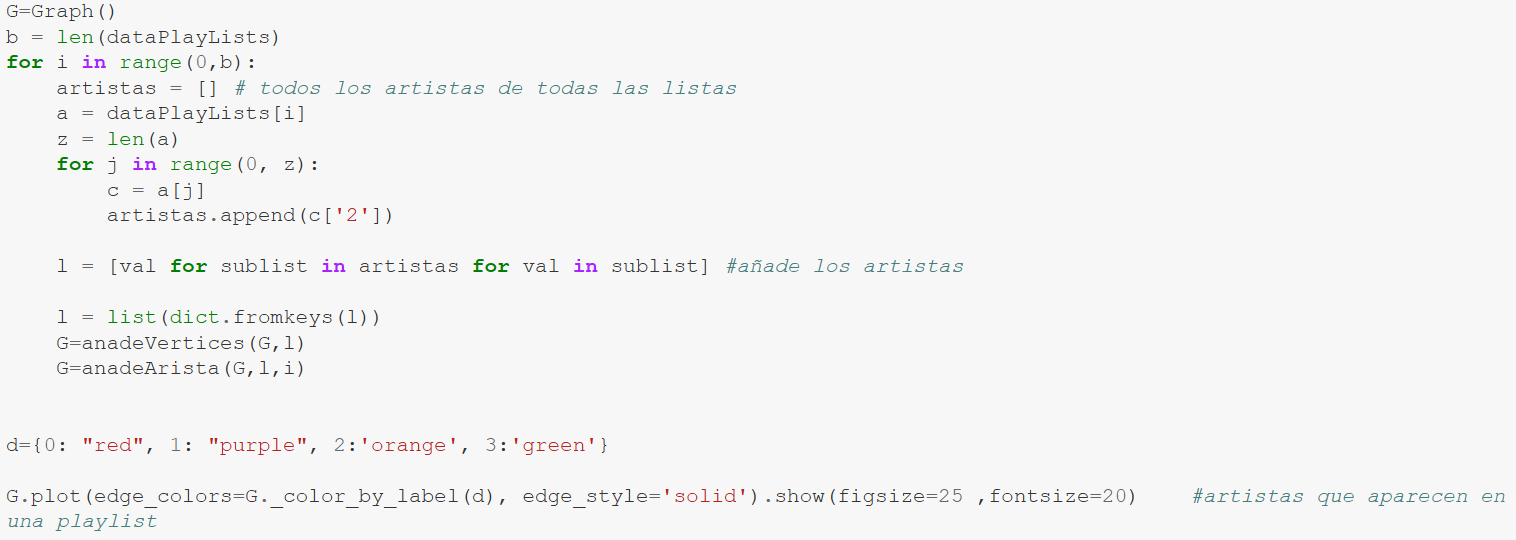
\includegraphics[width=0.7\textwidth]{sage_4.png}
	   }\\ %  ------- End of the first row ----------------------%
	   \subfigure[grafo]{%
		   \label{fig:third}
		   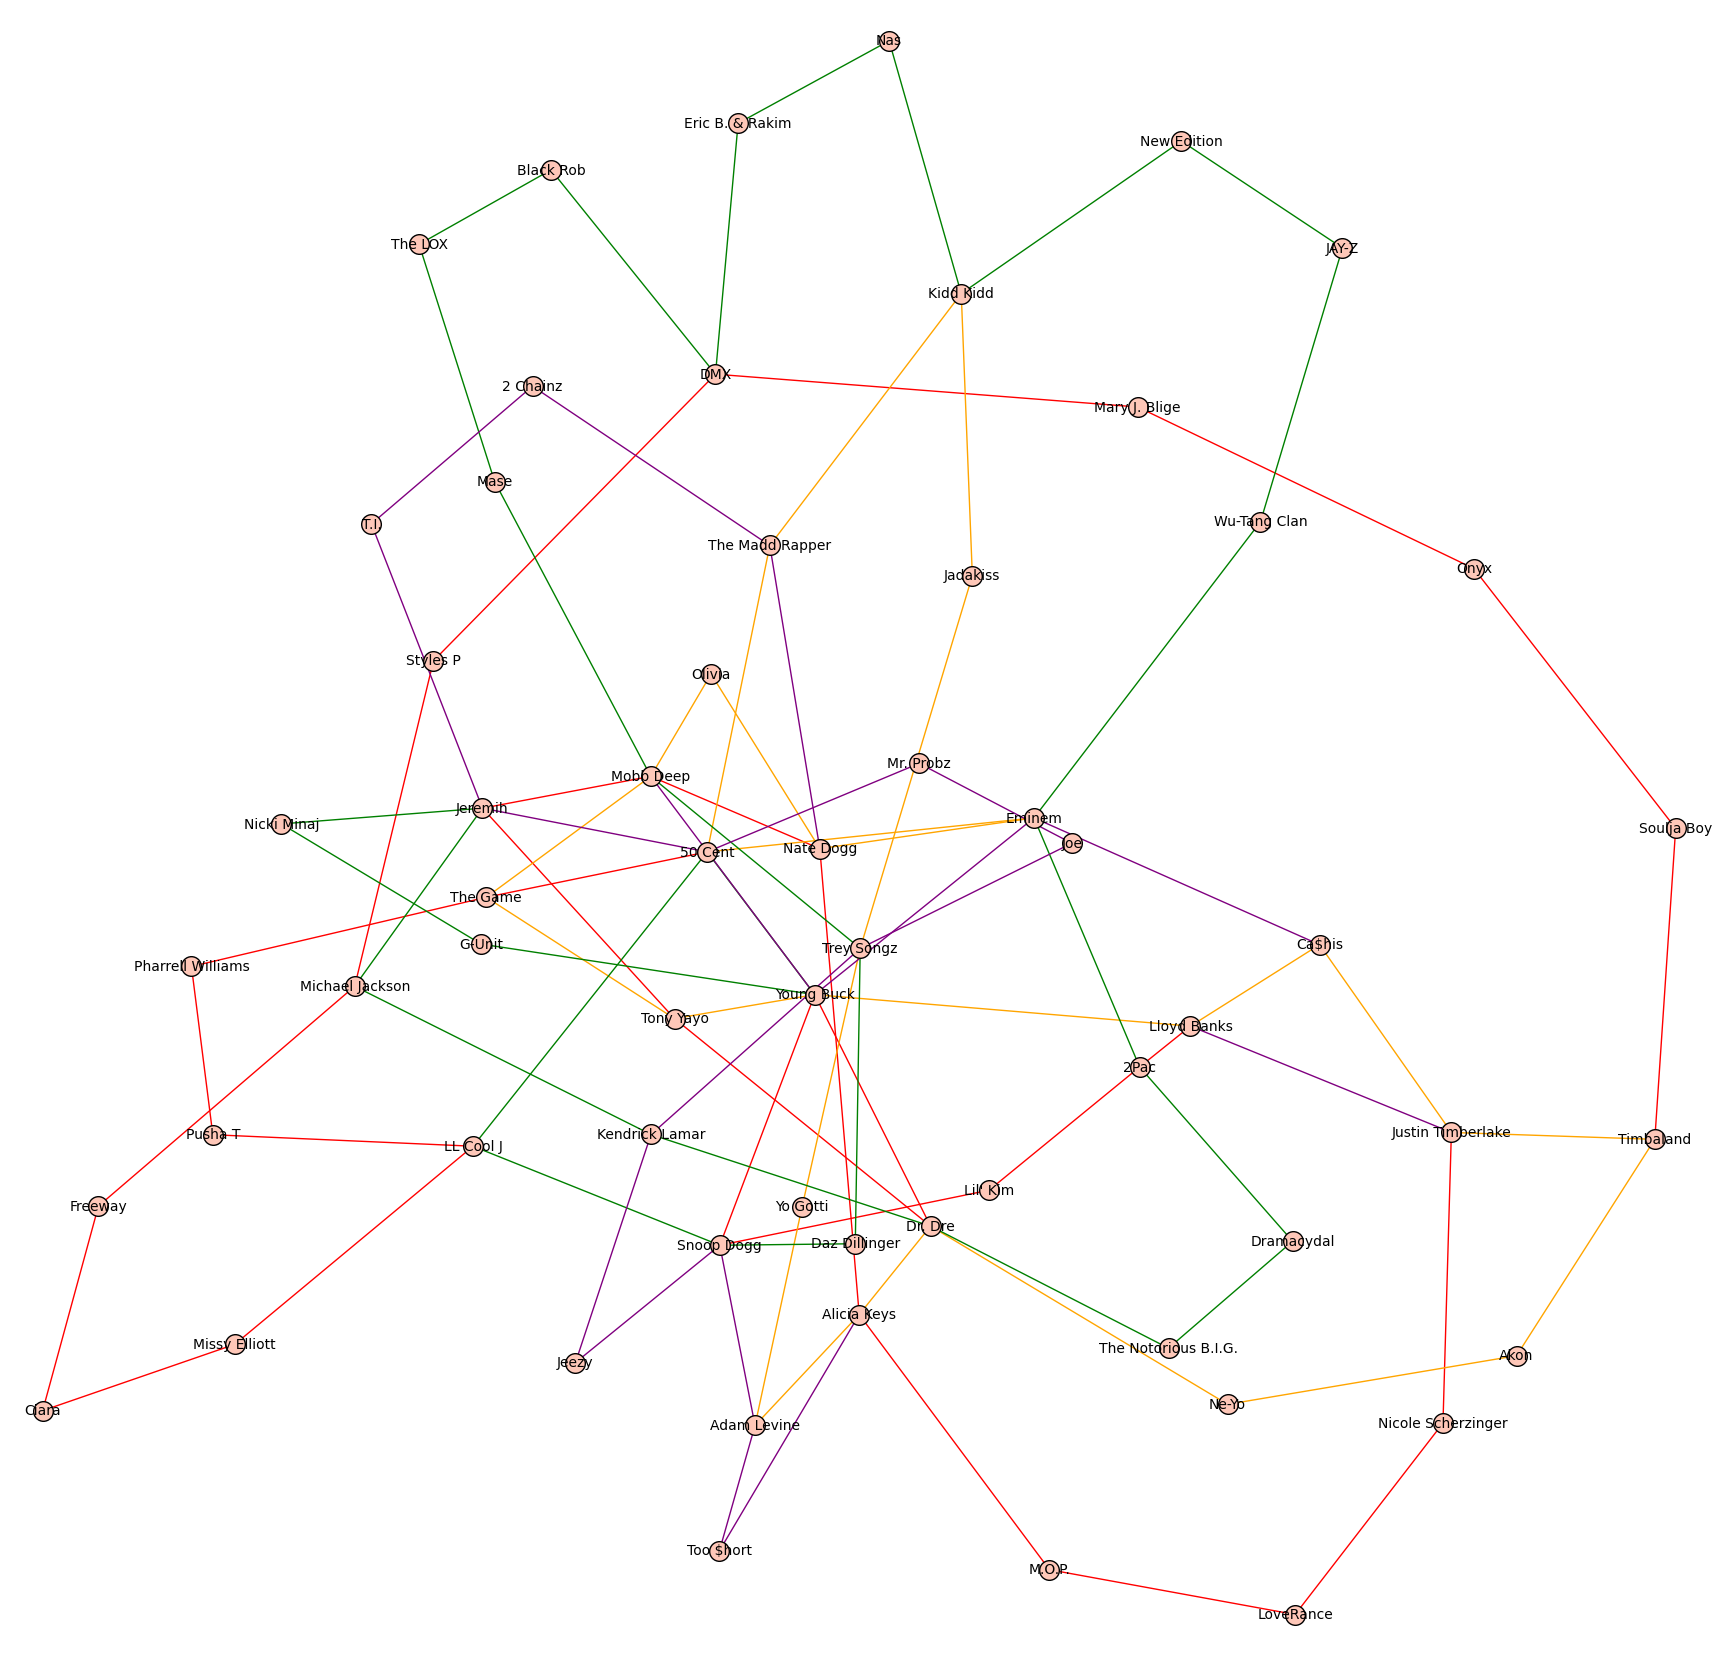
\includegraphics[width=0.7\textwidth]{sage_6.png}
	   }%
	  
%
	\end{center}
	\caption{%
	Código SageMath 2
 	}%
	\label{fig:codigoSage2}
\end{figure}


\paragraph*{De los artistas que participan en las playlists se han obtenido 
los mas populares por cada playlists, del mas popular se puede ver que Eminen es el ganador. Figura~\ref{fig:codigoSage3}.}

\paragraph*{Se pueden observar las comunidades segun los generos por artista, 
de las playlist anteriores podemos enconrar que los generos raiz son el hiphop y el rap
y podemos encontrar generos derivados como el nashville hip hop o el electropop. Figura~\ref{fig:codigoSage3}.}

\paragraph*{La centralidad de intermediacion nos permite detectar 
aquellos nodos que hacen de puente para otros nodos de tal forma que el camino se hace mas corto.
En este grafo tras aplicar la centralidad de intermediacion y coger los valores mas altos 
podemos observar que los mas importantes son Young Buck y 50 cent, 
curioso ya que 50 cent esta en todas las playlists. Figura~\ref{fig:codigoSage4}.}

\paragraph*{Practicamente coincide con el centro del grafo(cercania) Figura~\ref{fig:codigoSage4}.}

\paragraph*{Lo sorpredente de esta centralidad de grado es que a pesar de que 50cent es nuestro 
autor de estudio Mobb Deep tiene la misma centralidad de grado. Figura~\ref{fig:codigoSage4}.}


\begin{figure}[H]
	\begin{center}
%
	   \subfigure[Popularidad total según playlist]{%
		   \label{fig:first}
		   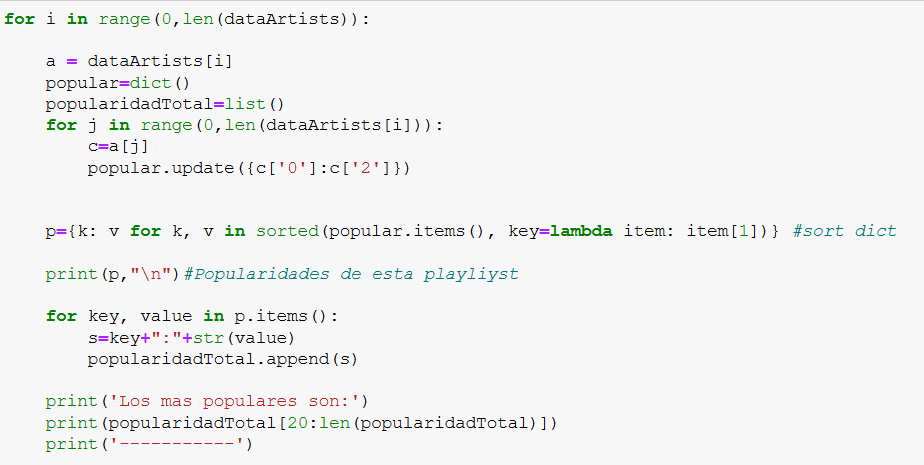
\includegraphics[width=0.5\textwidth]{sage_7.png}
	   }%
	   \subfigure[Salida popularidad total según playlist]{%
		   \label{fig:second}
		   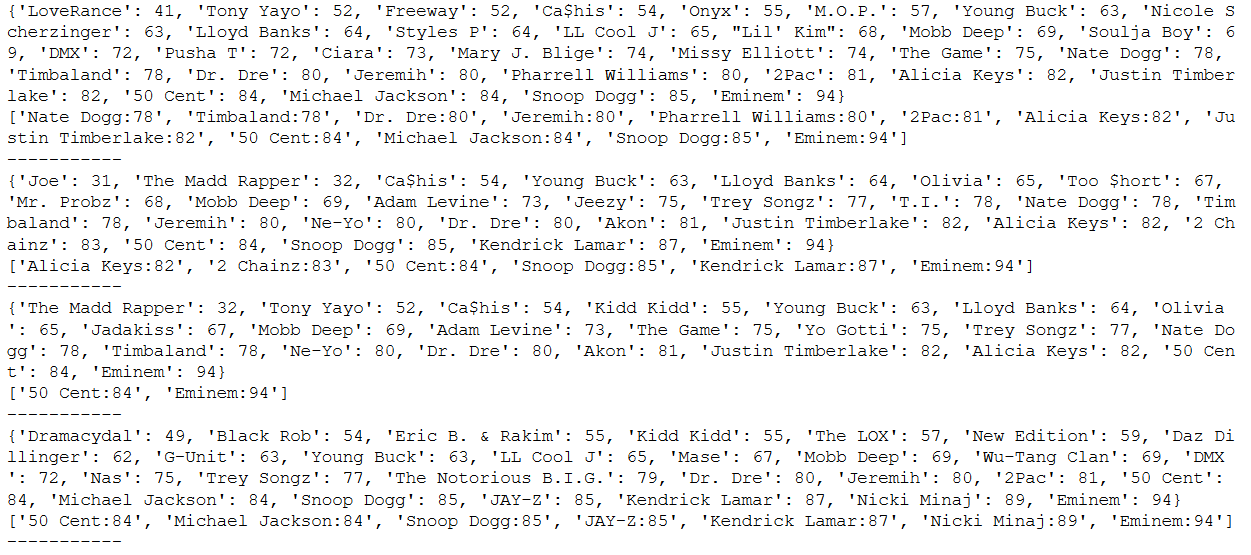
\includegraphics[width=0.5\textwidth]{sage_7_out.png}
	   }\\ %  ------- End of the first row ----------------------%
	   \subfigure[Género mas popular según playlist]{%
		   \label{fig:third}
		   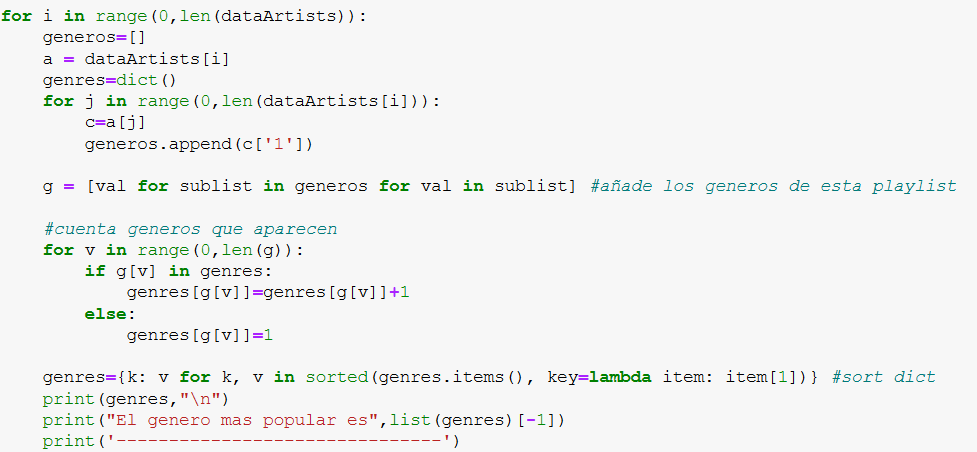
\includegraphics[width=0.5\textwidth]{sage_8.png}
	   }%
	   \subfigure[Salida Género mas popular según playlist]{%
		   \label{fig:four}
		   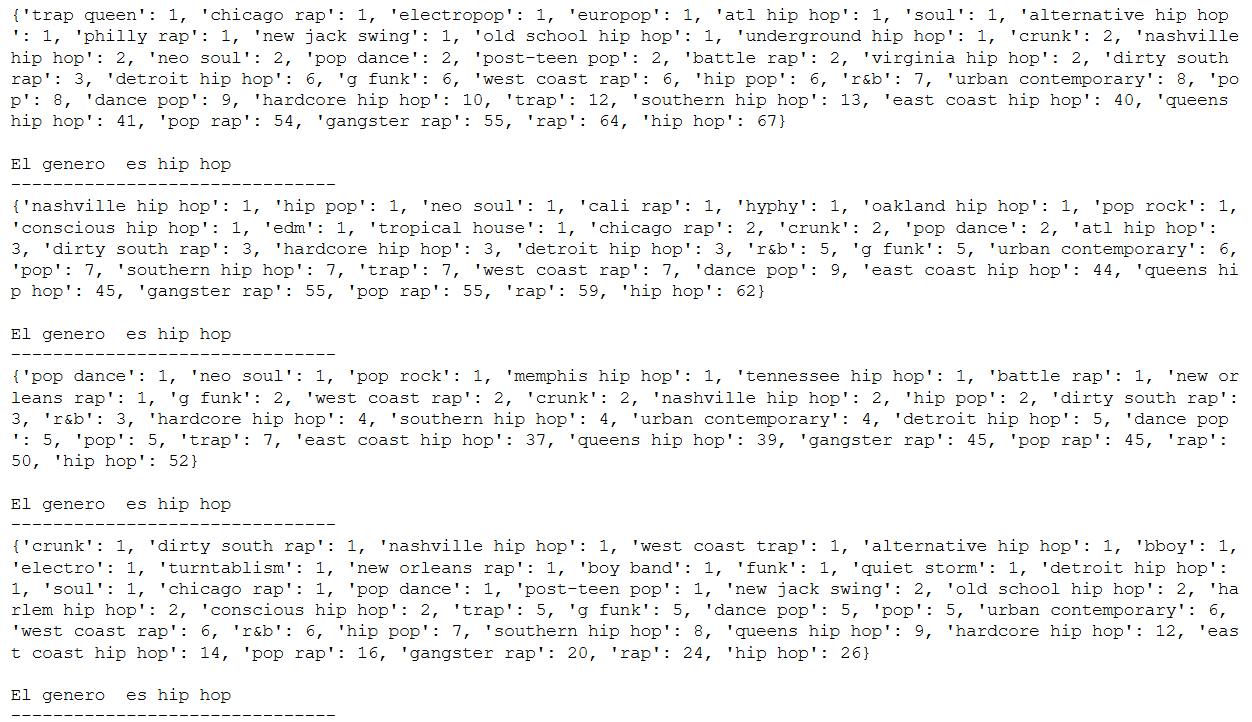
\includegraphics[width=0.5\textwidth]{sage_8_out.png}
	   }%
%
	\end{center}
	\caption{%
	Código SageMath 3
 	}%
	\label{fig:codigoSage3}
\end{figure}

\pagebreak

\begin{figure}[H]
	\begin{center}
%
	   \subfigure[Centralidad de grado]{%
		   \label{fig:first}
		   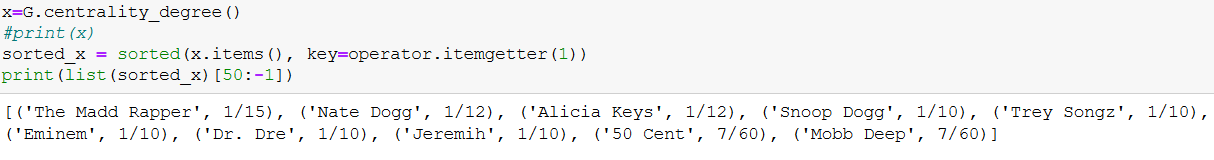
\includegraphics[width=1.0\textwidth]{sage_11.png}
	   }\\%  ------- End of the first row ----------------------%
	   \subfigure[Centralidad de intermediación]{%
		   \label{fig:second}
		   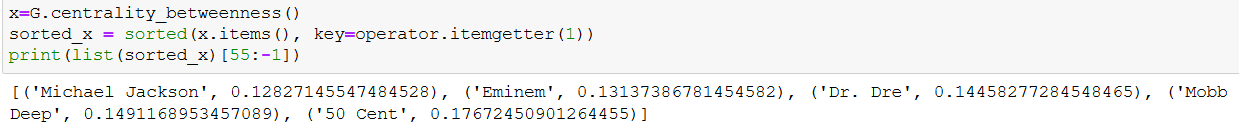
\includegraphics[width=1.0\textwidth]{sage_9.png}
	   }\\ %  ------- End of the first row ----------------------%
	   \subfigure[Centralidad de cercanía]{%
		   \label{fig:third}
		   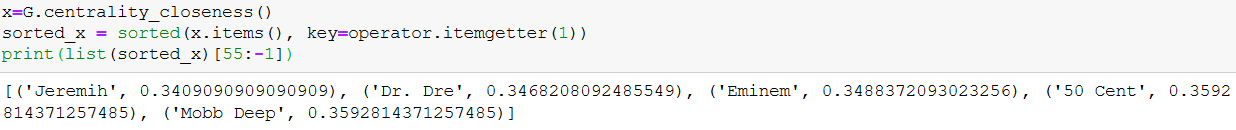
\includegraphics[width=1.0\textwidth]{sage_10.png}
	   }%
%
	\end{center}
	\caption{%
	Código SageMath 4
 	}%
	\label{fig:codigoSage4}
\end{figure}

\paragraph*{Ahora veremos el estudio de comunidades para ello hemos utilizado los metódos realizados en la práctica de comunidades de la asignatura. Figura~\ref{fig:codigoSage5}.}

\begin{figure}[H]
	\begin{center}
%
	   \subfigure[Similitud]{%
		   \label{fig:first}
		   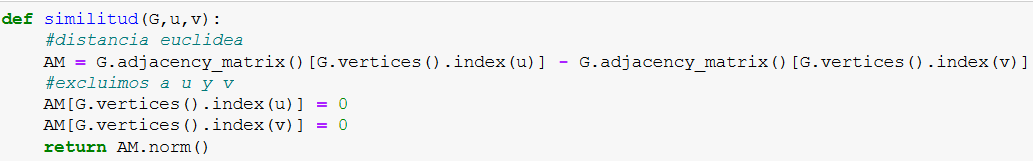
\includegraphics[width=0.5\textwidth]{sage_12.png}
	   }%
	   \subfigure[Similitud entre comunidades]{%
		   \label{fig:second}
		   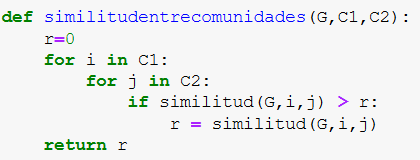
\includegraphics[width=0.5\textwidth]{sage_13.png}
	   }\\ %  ------- End of the first row ----------------------%
	   \subfigure[Unir comunidades]{%
		   \label{fig:third}
		   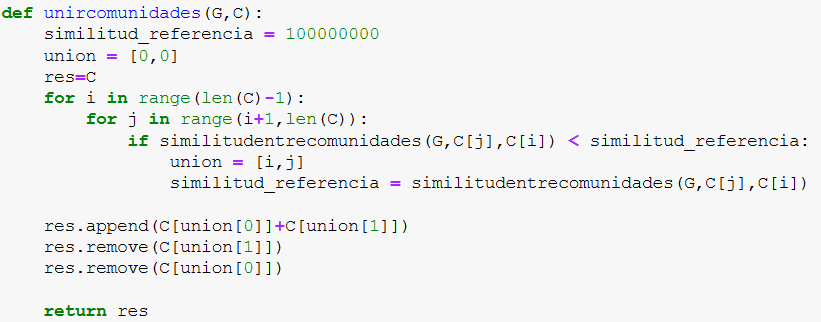
\includegraphics[width=0.5\textwidth]{sage_14.png}
	   }%
	   \subfigure[Comunidades aplicando modularidad]{%
		   \label{fig:four}
		   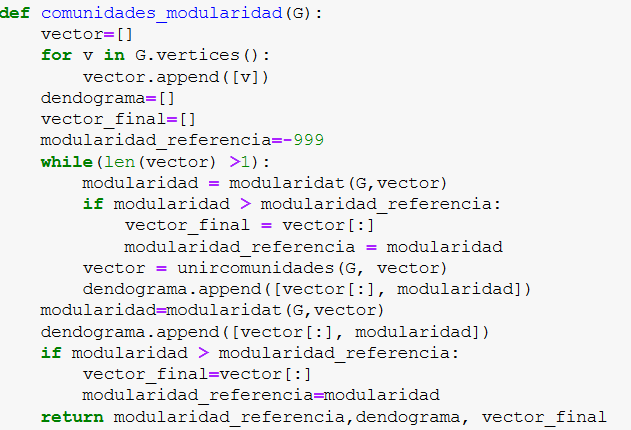
\includegraphics[width=0.5\textwidth]{sage_15.png}
	   }%
%
	\end{center}
	\caption{%
	Código SageMath 5
 	}%
	\label{fig:codigoSage5}
\end{figure}

\paragraph*{La modularidad nos permite enconrar aquellos nodos que tienen una conexion muy fuerte con sus vecinos, 
y el algoritmo Hierarchical clustering nos permite encontrar esas 8 comunidades.Figura~\ref{fig:codigoSage6}.}
\begin{figure}[H]
	\begin{center}
%
	   \subfigure[Salida comunidades]{%
		   \label{fig:first}
		   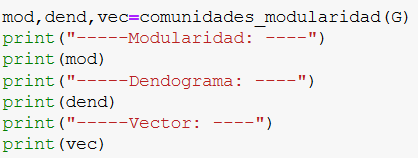
\includegraphics[width=0.5\textwidth]{sage_16.png}
	   }%
	   \subfigure[Vector de comunidades]{%
		   \label{fig:second}
		   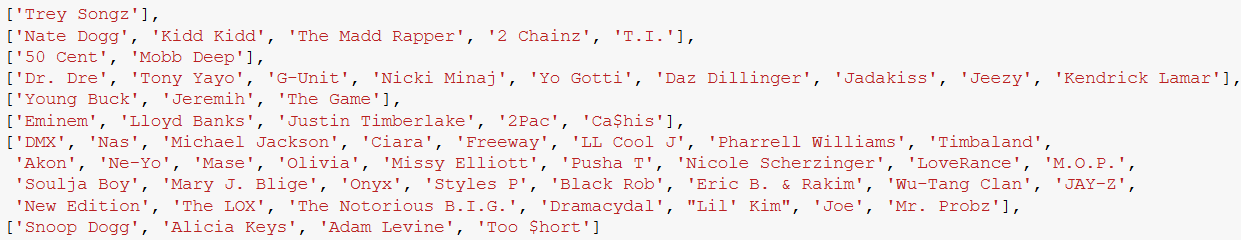
\includegraphics[width=0.5\textwidth]{sage_17.png}
	   }
	   
%
	\end{center}
	\caption{%
	Código SageMath 6
 	}%
	\label{fig:codigoSage6}
\end{figure}


\section{Conclusiones}

\paragraph*{A diferencia de otras redes como Twitter o Facebook, Spotify es un tanto más difícil de estudiar ya que no es tan susceptible de que un ojo novato cree con poco esfuerzo un boceto de como funcionan las relaciones entre artistas, 
no como en Facebook que con ir diciendo premisas como "Fulanito es amigo de Pepito, así que puedo unirlos con una arista, y entonces...", o "Naranjito le dio retweet a Manolito, así que puedo relacionarlos con una arista, y entonces...", obtener una red es asequible. Spotify te puede ofrecer en cambio listas de reproducción con ciertos artistas, álbumes de esos artistas e incluso podcasts, lo que hace que el ojo inexperto tenga problemas para buscar una forma de estudiar la red. }

\paragraph*{Sin embargo, al estudiar a un artista en concreto como 50 Cent a partir de sus listas de reproducción, hemos obtenidos resultados interesantes, como que por ejemplo él no sea el artista más famoso de su grupo, sino Eminem, o que por ejemplo un artista Mobb Deep sea un artista de paso entre todas las listas de reproducción.
Todos estos resultados fueron gratificantes y cuanto menos informativos del comportamiento de Spotify.}


\end{document}
